\chapter{МЕТОДОЛОГИЯ МНОГОКРИТЕРИАЛЬНОЙ ОПТИМИЗАЦИИ ПАРАМЕТРОВ ПНЕВМОПРИВОДА}\label{ch:ch4}

Задача многокритериальной оптимизации параметров пневмопривода
заключается в нахождении оптимального набора параметров системы
управления, обеспечивающего баланс между несколькими конфликтующими
критериями качества работы привода. Основными критериями в данном случае
выступают точность позиционирования выходного звена пневмопривода и
частота переключений дискретных пневмораспределителей, которые определяют
долговечность и энергопотребление системы. Оптимизация параметров управления
направлена на минимизацию ошибок позиционирования при минимально возможном числе
переключений, что позволяет продлить срок службы оборудования и снизить износ компонентов.

\section{Последовательность решения задачи многокритериальной оптимизации параметров пневмопривода}\label{ch:ch4/sec1}

Решение задачи многокритериальной оптимизации параметров электропневматического привода осуществляется в соответствии с
предложенной методологией, включающей следующие основные этапы.
На первом этапе производится формализация целевых
функций оптимизации. Вводится вектор критериев качества:
\begin{equation}
\mathbf{J}(\mathbf{p}) = \begin{bmatrix}
J_1(\mathbf{p}) \
J_2(\mathbf{p})
\end{bmatrix} = \begin{bmatrix}
\frac{1}{T}\sum_{i=1}^{4}N_i \
\int_0^T (x_{\text{зад}} - x(t))^2 dt
\end{bmatrix}
\end{equation}
где $\mathbf{p}$ -- вектор оптимизируемых параметров алгоритма управления;
$N_i$ -- количество переключений $i$-го распределителя;
$T$ -- время наблюдения;
$x_{\text{зад}}$ -i заданное положение;
$x(t)$ -- текущее положение штока.

Далее осуществляется определение пространства параметров:
\begin{equation}
\mathbf{p} \in \mathcal{P} = {\mathbf{p} \in \mathbb{R}^d: \mathbf{p}{\text{min}} \leq \mathbf{p} \leq \mathbf{p}{\text{max}}}
\end{equation}
где $d$ -- размерность вектора параметров;
$\mathbf{p}{\text{min}}$, $\mathbf{p}{\text{max}}$ -- векторы минимальных и максимальных значений параметров.

На втором этапе формируется начальная выборка точек в пространстве параметров
методом латинского гиперкуба, обеспечивающим равномерное покрытие области
поиска. Для каждой точки выборки проводится численное моделирование системы и вычисляются значения критериев качества.
Процесс этапа схематически представлен на рисунке \ref{fig:step_2_scheme}.

\begin{figure}[ht]
    \centerfloat{
    \includegraphics{part4/step_2_scheme.pdf}
    }
    \caption{Схема второго этапа методологии многокритериальной оптимизации.}\label{fig:step_2_scheme}
\end{figure}


Третий этап заключается в построении суррогатных моделей для аппроксимации зависимостей критериев качества от параметров:
\begin{equation}
\hat{J}_i(\mathbf{p}) = f_i(\mathbf{p}, \mathbf{w}_i), \quad i = 1,2
\end{equation}
где $f_i$ -- функция суррогатной модели;
$\mathbf{w}_i$ - вектор параметров модели.

На четвертом этапе осуществляется поиск множества Парето-оптимальных
решений с использованием генетического алгоритма NSGA-II, оперирующего
суррогатными моделями. Фронт Парето формируется как множество недоминируемых решений:
\begin{equation}
\mathcal{P}^* = {\mathbf{p} \in \mathcal{P}: \nexists \mathbf{p}' \in \mathcal{P}, \mathbf{J}(\mathbf{p}') \preceq \mathbf{J}(\mathbf{p})}
\end{equation}

Пятый этап включает верификацию полученных решений путем численного моделирования
системы с выбранными параметрами и уточнение суррогатных моделей в окрестности фронта Парето.

На заключительном этапе производится анализ полученных результатов,
выявление характерных областей фронта Парето и формирование
рекомендаций по выбору параметров алгоритма управления в зависимости от приоритетов между критериями качества.
Предложенная последовательность решения задачи многокритериальной оптимизации
обеспечивает эффективный поиск оптимальных параметров алгоритма
управления электропневматическим приводом с учетом компромисса
между точностью позиционирования и частотой переключений распределителей.

Применение суррогатных моделей позволяет существенно сократить вычислительные затраты при сохранении требуемой точности оптимизации.

Рассмотрим в дальнейшем методы построения суррогатных моделей
и их применение в задаче оптимизации параметров управления пневмоприводом.
\section{Постановка задачи многокритериальной оптимизации параметров пневмопривода}\label{ch:ch4/sec2}

Для решения задачи применяются методы построения фронта Парето,
позволяющие выделить множество неулучшаемых решений, представляющих
компромисс между критериями. Оптимизационная задача формулируется как
поиск таких значений параметров управления, при которых улучшается
один из критериев, не ухудшая при этом другие. Это достигается путем
численного моделирования системы с использованием суррогатных моделей,
которые сокращают вычислительные затраты и позволяют быстро оценивать
показатели качества при различных сочетаниях параметров. Результаты
оптимизации используются для выбора наилучшей стратегии управления
пневмоприводом в зависимости от заданных условий эксплуатации и
требований к точности и ресурсам системы.

\subsection{Концепция оптимальности по Парето}\label{ch:ch4/sec2/subsec1}

Концепция оптимальности по Парето, предложенная итальянским экономистом
Вильфредо Парето \cite*{pareto1896cours} в конце XIX века, является фундаментальным понятием в теории
многокритериальной оптимизации. Данная концепция предоставляет математический аппарат для
анализа и принятия решений \cite*{miettinen1999nonlinear} в ситуациях, где необходимо одновременно оптимизировать несколько,
зачастую противоречивых, критериев.

Рассмотрим задачу многокритериальной оптимизации с $k$ целевыми функциями \cite*{deb2001multi}:

\begin{equation}
    \label{eq:multiobjective_optimization}
    \min_{x \in \Omega} F(x) = (\min f_1(x), \min f_2(x), \ldots, \min f_k(x)),
\end{equation}
где $x \in \Omega \subset \mathbb{R}^n$ -- вектор решений, принадлежащий допустимому множеству $\Omega$;
$F: \Omega \rightarrow \mathbb{R}^k$ -- векторная целевая функция.

Решение $x^* \in \Omega$ называется оптимальным по Парето
(или Парето-оптимальным), если не существует другого решения $x \in \Omega$, такого что:

\begin{equation}
    \begin{cases}
        \forall i \in \{1, \ldots, k\}: f_i(x) \leq f_i(x^*), \\
        \exists j \in \{1, \ldots, k\}: f_j(x) < f_j(x^*).
    \end{cases}
\end{equation}

Иными словами, решение является Парето-оптимальным, если невозможно
улучшить значение любого критерия без ухудшения значения хотя бы одного другого критерия.

Концепция оптимальности по Парето тесно связана с понятием доминирования.
Говорят, что решение $x_1$ доминирует решение $x_2$ (обозначается как $x_1 \prec x_2$), если выполняются следующие условия:

\begin{equation}
    \label{eq:dominance}
    \begin{cases}
        \forall i \in \{1, \ldots, k\}: f_i(x_1) \leq f_i(x_2), \\
        \exists j \in \{1, \ldots, k\}: f_j(x_1) < f_j(x_2).
    \end{cases}
\end{equation}

Множество всех Парето-оптимальных решений образует множество
недоминируемых решений, которое также называется множеством Парето или Парето-множеством.

Образ множества Парето в пространстве критериев называется фронтом Парето. Математически фронт Парето можно определить как:

\begin{equation}
    PF = \{F(x) | x \in PS\},
\end{equation}
где $PS$ -- множество Парето в пространстве решений.

Фронт Парето представляет собой геометрическое место точек \cite*{coello2007evolutionary} в
пространстве критериев, соответствующих недоминируемым решениям.
Он наглядно демонстрирует компромиссы между различными целевыми
функциями и играет ключевую роль в процессе принятия решений.

На рисунке \ref{fig:pareto_front_example} приведен пример фронта Парето для двух критериев.

\begin{figure}[ht]
    \centerfloat{
    \includegraphics{part4/pareto_front_demonstrate.pdf}
    }
    \caption{Пример фронта Парето для двух критериев.}\label{fig:pareto_front_example}
\end{figure}[ht]

На рисунке видно, что фронт Парето представляет собой кривую, состоящую из
недоминируемых решений
(точек), для которых невозможно улучшить один критерий без ухудшения другого.

Основные свойства оптимальности по Парето:
\begin{enumerate}
    \item Несравнимость: Парето-оптимальные решения несравнимы между собой в смысле доминирования.

    \item Иерархическая структура: Концепция Парето-оптимальности может быть расширена на случай иерархической оптимизации, где критерии имеют различные приоритеты.

    \item Инвариантность: Парето-оптимальные решения инвариантны относительно монотонных преобразований целевых функций.

    \item Выпуклость: Если все целевые функции выпуклы и допустимое множество выпукло, то множество Парето также выпукло.
\end{enumerate}

Для нахождения множества Парето-оптимальных решений в задачах многокритериальной оптимизации
используются специальные эволюционные алгоритмы. Эти методы работают с популяциями решений и
постепенно улучшают их, используя механизмы, подобные естественному отбору. Ниже описаны два из наиболее
известных алгоритмов для поиска Парето-оптимальных решений.

Сущществует множество методов для поиска Парето-оптимальных решений, однако наиболее
распространенными являются эволюционные алгоритмы, такие как NSGA-II и SPEA2.

NSGA-II — это один из самых популярных эволюционных алгоритмов для многокритериальной оптимизации. Его ключевые особенности:

\begin{enumerate}
    \item Сортировка по доминированию: На каждом шаге алгоритм делит популяцию на несколько уровней,
    исходя из степени доминирования решений. Те решения, которые не доминируются другими, попадают в
    первый уровень, остальные сортируются в соответствии с их степенью доминирования.

    \item Crowding Distance: NSGA-II использует метрику "crowding distance" для оценки плотности
    решений в области фронта Парето. Это помогает поддерживать разнообразие решений, предотвращая
    их слияние в одном месте.

    \item Операторы отбора, скрещивания и мутаций: Алгоритм применяет стандартные операторы
    генетического алгоритма для эволюции популяции — отбор лучших решений, скрещивание и мутацию
    для создания нового поколения.
\end{enumerate}

NSGA-II обеспечивает эффективное нахождение множества Парето-оптимальных решений,
а также хорошо сохраняет разнообразие решений вдоль фронта Парето \cite*{deb2001multi}.

SPEA2 — это улучшенная версия алгоритма SPEA, разработанная для повышения эффективности поиска недоминируемых решений. Основные улучшения SPEA2 включают:

\begin{enumerate}
    \item Архивирование решений: SPEA2 сохраняет архив недоминируемых решений на каждом шаге, что помогает гарантировать,
    что фронт Парето не будет потерян в процессе эволюции.

    \item Оценка решений: Каждый элемент популяции получает оценку на основе того,
    сколько решений он доминирует и насколько сильно доминируется сам. Эта оценка
    используется для выбора кандидатов для следующего поколения.

    \item Учет плотности решений: Подобно NSGA-II, SPEA2 учитывает плотность решений
    вблизи каждого кандидата, что помогает поддерживать разнообразие и улучшать
    распределение решений вдоль фронта Парето.
\end{enumerate}

SPEA2 продемонстрировал высокую производительность на сложных задачах многокритериальной
оптимизации и может эффективно находить множество недоминируемых решений \cite{zitzler2001spea2}.

В задаче оптимизации параметров управления пневматическим приводом концепция оптимальности
по Парето позволяет учесть множественные, зачастую противоречивые, критерии качества управления.
Например, минимизация времени переходного процесса и минимизация колличества переключений распределителей
могут находиться в конфликте друг с другом. Построение фронта Парето в этом случае
позволяет выявить множество оптимальных компромиссных решений и
предоставить лицу, принимающему решения, полную картину возможных вариантов.
\section{Методы построения сурогантных моделей}\label{sec:ch4/sec3}
Суррогатное моделирование является достаточно эффектиынвм методом в
задачах многокритериальной оптимизации, особенно при построении
Парето-фронта. Как правило, оно используется для аппроксимации сложных и вычислительно
затратных функций или систем, что позволяет значительно снизить временные и вычислительные
затраты на решение задач, требующих многократной оценки целевых функций. Данный
подход особенно полезен в тех случаях, когда каждая отдельная оценка целевой функции
является дорогостоящей с точки зрения времени или ресурсов, как это часто встречается
при численном моделировании физических процессов или компьютерных симуляциях сложных
инженерных систем.

Для синжения Для снижения вычислительных затрат используется суррогатное моделирование,
при котором сложные функции аппроксимируются с помощью более простых моделей,
называемых суррогатами, которые можно быстро и эффективно вычислять.
Это позволяет оптимизировать процесс поиска Парето-фронта и находить решения
с меньшими затратами ресурсов.



\subsection{Обзор методов суррогатного моделирования}\label{sec:ch4/sec3/subsec1}


\paragraph{Полиномиальная регрессия}\label{sec:ch4/sec3/subsec1/subsubsec1}

Полиномиальная регрессия представляет собой метод аппроксимации данных
с использозванием полиномов различных степеней. Этот метод является расширением линейной
регрессии и позволяет моделировать зависисмости между входными и выходными переменными более
гибким образом, используя дополнительные нелинейные термины, такие как квадратичные, кубические члены
и~т.д., а также их взаимодействия \cite{fan2018local}.

Полиномиальная регрессия предполагает, что зависимость между предикторами и откликом
можеты быть описана полиноминальной функцией вида:

\begin{equation}
    \hat{y}(\mathbf{x}) = \beta_0 + \sum_{i=1}^{p} \beta_i x_i + \sum_{i=1}^{p} \sum_{j=1}^{p} \beta_{ij} x_i x_j + \ldots,
\end{equation}
где $\hat{y}(\mathbf{x})$ -- предсказанное значение отклика;
$\beta_0$ -- свободный член (интерцепт);
$\beta_i$ -- коэффициенты линейных членов $x_i$;
$\beta_{ij}$ -- коэффициенты взаимодействия между переменными $x_i$ и $x_j$;
$p$ -- количество перменных;
$x_i,~x_j$ -- входные переменные.

Для случая квадратичной регрессии полиноминальная функция принимает вид:

\begin{equation}
    \hat{y} = \beta_0 + \beta_1 x_1 + \beta_2 x_2 + \beta_3 x_1^2
    + \beta_4 x_2^2 + \beta_5 x_1 x_2.
\end{equation}

Здесь учитываются коэффициенты линейных $\beta_1,~\beta_2$ и квадратичных $\beta_3,~\beta_4$ членов,
а также коэффициент взаимодействия $\beta_5$ \cite{heiberger2009polynomial}.

Для определения коэффициентов $\beta$ используется метод наименьших квадратов,
который минимизирует сумму квадратов отколнений между наблюдаемыми значениям $y_i$
и предсказанными $\hat{y}_i$. Задача оптимизации формулируется следующим образом:

\begin{equation}
    \min_{\beta} \sum_{i=1}^{n} (y_i - \hat{y}_i)^2 =
    \min_{\beta} \sum_{i=1}^{n} \left\{
    y_i - \left(\beta_0 + \sum_{j=1}^{p} \beta_j x_{ij}
    + \sum_{j=1}^{p} \sum_{k=1}^{p} \beta_{jk} x_{ij} x_{ik}
    \right)
    \right\}^2,
\end{equation}
где $n$ -- количество наблюдений.

Для решения этой задачи вводится матричная форма:

\begin{equation}
    \mathbf{y} = \mathbf{X} \boldsymbol{\beta} + \boldsymbol{\epsilon},
\end{equation}
где $\mathbf{y}$ -- вектор наблюдаемых значений откликов размерности $n \times 1$;
$\mathbf{X}$ -- матрица признаков размерности $n \times m$, где $m$ -- количество коэффициентов,
включая взаимодействия и нелинейные члены;
$\boldsymbol{\beta}$ -- вектор коэффициентов размерности $m \times 1$;
$\boldsymbol{\epsilon}$ -- вектор ошибок.

Оценка коэффицикнтов $\boldsymbol{\beta}$ производится с использованием псевдообратной матрицы:
\begin{equation}
    \boldsymbol{\beta} = (\mathbf{X}^T \mathbf{X})^{-1} \mathbf{X}^T \mathbf{y}.
\end{equation}
где $(\mathbf{X}^T \mathbf{X})^{-1} \mathbf{X}^T$ -- псевдообратная матрица Мура-Пенроуза,
которая обеспечивает минимизацию ошибки на оценке коэффициентов \cite{meyer2009matrix}.

Преимущества полиномиальной регрессии для задачи оптимизации управления электропневматическими приводами:
\begin{enumerate}
    \item Простота реализации и интерпретации модели.
    \item Низкие вычислительные затраты на построение и использование модели.
    \item Возможность аналитического вычисления градиентов, что полезно для оптимизационных алгоритмов.
\end{enumerate}

Ограничения метода:
\begin{enumerate}
    \item Ограниченная способность моделировать сложные нелинейные зависимости, характерные для пневматических систем;
    \item Риск переобучения при использовании полиномов высоких степеней;
    \item Чувствительность к выбросам в экспериментальных данных.
\end{enumerate}

\paragraph{Радиальные базисные функции}\label{sec:ch4/sec3/subsec1/subsubsec2}


Преимущества метода RBF:

\begin{enumerate}
    \item Способность эффективно аппроксимировать сложные нелинейные зависимости.
    \item Хорошая обобщающая способность при правильном выборе параметров.
    \item Возможность точной интерполяции в экспериментальных точках.
\end{enumerate}

Ограничения метода:

\begin{enumerate}
    \item Чувствительность к выбору параметров (количество и расположение центров, тип базисной функции, параметр формы).
    \item Потенциальные проблемы с обусловленностью матрицы интерполяции при большом количестве базисных функций.
    \item Сложность интерпретации модели по сравнению с полиномиальной регрессией.
\end{enumerate}

\paragraph{Гауссовы процессы (Кригинг)}\label{sec:ch4/sec3/subsec1/subsubsec3}

Кригинг (Гауссовы процессы) является мощным методом интерполяции,
который позволяет строить суррогатные модели для сложных функций,
используя концепцию случайных процессов \cite{gramacy2020surrogates}. Он основан
на предположении, что процесс \( y(\mathbf{x}) \) может быть представлен в виде:

\begin{equation}
    y(\mathbf{x}) = \mu + Z(\mathbf{x}),
\end{equation}
где $\mu$ -- среднее значение; $Z(\mathbf{x})$ -- гауссовский процесс с нулевым средним и
ковариационной функцией \cite{marrel2024probabilistic}:

\begin{equation}
    \text{Cov}(Z(\mathbf{x}_i), Z(\mathbf{x}_j)) = k(\mathbf{x}_i, \mathbf{x}_j),
\end{equation}

Ковариационная функция часто задается как радиальная базисная функция:

\begin{equation}
    k(\mathbf{x}_i, \mathbf{x}_j) = \sigma^2 \exp\left(-\frac{\|\mathbf{x}_i - \mathbf{x}_j\|^2}{2l^2}\right),
\end{equation}.
где \( \sigma^2 \) — дисперсия;
$l$ — параметр длины \cite{figueroa2021gaussian}.

Предсказание значений в новых точках $\mathbf{x}_*$ осуществляется через условное распределение, учитывающее известные значения.
Среднее предсказание и его дисперсия определяются как:

\begin{equation}
    \hat{y}(\mathbf{x}_*) = \mu + \mathbf{k}_*^T \mathbf{K}^{-1} (\mathbf{y} - \mu \mathbf{1}_n),
\end{equation}

\begin{equation}
    \text{Var}(\hat{y}(\mathbf{x}_*)) = k(\mathbf{x}_*, \mathbf{x}_*) - \mathbf{k}_*^T \mathbf{K}^{-1} \mathbf{k}_*,
\end{equation}
где $\mathbf{k}_*$ — вектор ковариаций между новой точкой и обучающими точками;
$\mathbf{K}$ — ковариационная матрица \cite{zhou2020enhanced}.

Кригинг широко применяется в задачах многокритериальной оптимизации и позволяет
не только предсказывать значения, но и оценивать их неопределенность, что особенно
полезно при построении фронтов Парето и выборе компромиссных решений \cite{radaideh2020surrogate}.

Преимущества метода кригинга:

\begin{enumerate}
    \item Высокая точность интерполяции и экстраполяции;
    \item Возможность оценки неопределенности предсказаний;
    \item Гибкость в моделировании сложных нелинейных зависимостей;
    \item Эффективность при ограниченном количестве экспериментальных данных.
\end{enumerate}

Ограничения метода:

\begin{enumerate}
    \item Вычислительная сложность при большом количестве экспериментальных точек;
    \item Чувствительность к выбору функции корреляции и ее параметров;
    \item Сложность интерпретации модели по сравнению с детерминированными методами.
\end{enumerate}

\paragraph{Метод опорных векторов.}

Метод опорных векторов (SVM) представляет собой один из наиболее эффективных методов классификации и
регрессии, основанный на поиске гиперплоскости, которая максимизирует зазор между классами.
Основная идея заключается в преобразовании исходных данных в более
высокое измерение с целью нахождения разделяющей гиперплоскости \cite{Jakkula2006}.

Рассмотрим обучающую выборку:
\begin{equation}
    \{(x_i, y_i)\}_{i=1}^N,
\end{equation}
где $x_i \in \mathbb{R}^n$ -- вектор признаков;
$y_i \in \{-1, 1\}$ -- метка класса.

Задача заключается в нахождении гиперплоскости,
которая разделяет два класса с максимальным зазором. Гиперплоскость определяется уравнением:

\begin{equation}
    f(x) = w^T x + b = 0,
\end{equation}
где $w \in \mathbb{R}^n$ -- вектор весов;
$b \in \mathbb{R}$ -- смещение.

Целью является минимизация следующей функции потерь с учетом ограничений:

\begin{equation}
    \min_{w, b} \frac{1}{2} \|w\|^2,
\end{equation}
при условиях:

\begin{equation}
    y_i (w^T x_i + b) \geq 1, \quad i = 1, \ldots, N.
\end{equation}

Для решения данной задачи применяется метод множителей Лагранжа,
что приводит к следующей двойственной задаче \cite{Patle2013}:

\begin{equation}
    \max_{\alpha} \sum_{i=1}^N \alpha_i - \frac{1}{2} \sum_{i=1}^N \sum_{j=1}^N \alpha_i \alpha_j y_i y_j (x_i^T x_j),
\end{equation}
при ограничениях:

\begin{equation}
    \sum_{i=1}^N \alpha_i y_i = 0, \quad \alpha_i \geq 0, \quad i = 1, \ldots, N.
\end{equation}
где $\alpha_i$ -- множители Лагранжа, которые определяют вклад каждого образца в решение задачи.

Для повышения мощности метода используется преобразование исходных данных
в пространство более высокой размерности с помощью ядровых
функций

\begin{equation}
    K(x_i, x_j) = \phi(x_i)^T \phi(x_j),
\end{equation}
где $\phi(\cdot)$ — отображение в новое
пространство признаков.

Распространенные ядра включают линейное,
полиномиальное и гауссово (радиальное базисное) ядро \cite{Deris2011}:

\begin{itemize}
    \item Линейное: $K(x_i, x_j) = x_i^T x_j$;
    \item Полиномиальное: $K(x_i, x_j) = (x_i^T x_j + 1)^d$;
    \item Гауссово: $K(x_i, x_j) = \exp\left(-\frac{\|x_i - x_j\|^2}{2\sigma^2}\right)$.
\end{itemize}

Для работы с шумными данными вводится параметр регуляризации $C$,
который контролирует баланс между шириной зазора и ошибками классификации.
Оптимизационная задача в этом случае принимает вид \cite{Boswell2002}:

\begin{equation}
    \min_{w, b, \xi} \frac{1}{2} \|w\|^2 + C \sum_{i=1}^N \xi_i,
\end{equation}

при условиях:

\begin{equation}
    y_i (w^T x_i + b) \geq 1 - \xi_i, \quad \xi_i \geq 0, \quad i = 1, \ldots, N,
\end{equation}
где $\xi_i$ -- переменные, отвечающие за допущенные ошибки.

Преимущества метода опорных векторов: 

\begin{enumerate}
    \item Высокая обобщающая способность, особенно при ограниченном наборе обучающих данных;
    \item Эффективность в задачах с большим количеством входных параметров;
    \item Способность моделировать сложные нелинейные зависимости.
\end{enumerate}

Ограничения метода:

\begin{enumerate}
    \item - Вычислительная сложность обучения модели для больших наборов данных;
    \item Чувствительность к выбору ядерной функции и настройке гиперпараметров;
    \item Сложность интерпретации модели по сравнению с более простыми методами, такими как полиномиальная регрессия.
\end{enumerate}

\paragraph{Нейронные сети}\label{sec:ch4/sec3/subsec1/subsubsec5}

\paragraph{Эволюционные алгоритмы и метаэвристики}\label{sec:ch4/sec3/subsec1/subsubsec6}
Эволюционные алгоритмы и метаэвристики представляют собой группу методов оптимизации,
вдохновленных природными процессами.
Они основанны на принципа биологической эвлюции и предлагают подходы, такие как генетические алгоритмы,
алгоритмы роя частиц, иммунные алгоритмы и др., которые позволяют эффективно искать решения
в пространстве возможных параметров \cite{zhang2015comparision}.

Основная идея эволюционных алгоритмов заключается в имитации процесса естественного отбора,
где популяция решений обновляется с каждым шагом алгоритма, и только наилучшие решения
сохраняются для следующего поколения. Алгоритм начинается с инициализации популяции случайных
решений, где каждое решение представляет собой набор параметров управления. Далее, для каждой
особи в популяции оценивается функция приспособленности, которая определяет, насколько хорошо
решение выполняет поставленную задачу. На основе функции приспособленности отбираются лучшие
решения, которые подвергаются мутации и скрещиванию, чтобы создать новые решения, и процесс
повторяется до тех пор, пока не будет достигнута заданная точность или не исчерпаны
вычислительные ресурсы.

Математически, решение $\mathbf{x}$ оптимизируется с помощью эволюционного алгоритма, следуюя
процедуре:

\begin{equation}
    x^{t+1} = \text{ОТБОР} \left\{
    \text{МУТАЦИЯ} \left\{
    \text{СКРЕЩИВАНИЕ} \left\{
    x^t
    \right\}
    \right\}
    \right\},
\end{equation}
где $x^t$ -- текущее решение;
$x^{t+1}$ -- новое решение;
$\text{ОТБОР}$ -- процедура отбора лучших решений или решений с высокой приспособленностью;
$\text{МУТАЦИЯ}$ -- процедура случайного или направленного изменения решения;
$\text{СКРЕЩИВАНИЕ}$ -- процедура комбинирования решений для создания новых вариантов.

Основные элементы эволюционного алгоритма можно описать следующим образом:

\begin{enumerate}
    \item Инициализация популяции: создание случайной популяции решений $x_i,~i = 1, \ldots, N$;
    \item Оценка приспособленности: для каждого решения рассчитвыается функция приспособленности $f(x_i)$,
          определяющая качество решения;
    \item Отбор: выбор лучших решений для создания нового решения;
    \item Скрещивание и мутация: создаются новые решения путем комбинирования и изменения существующих;
    \item Замена: новые решения заменяют старые в популяции и процесс повторяется до достижения критерия останова.
\end{enumerate}

Основные трудности применения эволюционных алгоритмов заключается
в определении параметров алгоритма, таких как размер популяции, вероятность мутации и
скрещивания, а также в обеспечении достаточной вычислительной мощности для
обработки большого числа итераций.

Метаэврестические подходы, такие как алгоритмы роя частиц и методы имитации отжига,
дополняют эволлюционные алгоритмы, предоставляя дополнительные инструменты для
исследования пространства решений. Эти методы доказали свою эффективность в
решении задач многокритериальной оптимизации, где необходимо сбалансировать
несколько противоречивых показателей качества.

Например, алгоритмы роя частиц (PSO) имитируют поведение стаци, где каждый
агент (частица) премещается в пространтсве решений с учетом своей собственной
истории и информации, полученной от других агентов. Частица $i$ обновляет
свою скорость и положение следующим образом:

\begin{equation}
    \begin{aligned}
        v_i^{t+1} & = \omega v_i^t + c_1 r_1 (p_i^t - x_i^t) + c_2 r_2 (g^t - x_i^t), \\
        x_i^{t+1} & = x_i^t + v_i^{t+1},
    \end{aligned}
\end{equation}
где $\omega$ -- коэффициент инерции;
$c_1, c_2$ -- коэффициенты обучения;
$r_1, r_2$ -- случайные числа;
$p_i$ -- лучшее положение частицы;
$g$ -- лучшее положение частицы.

Преимущества эволюционных алгоритмов и метаэвристик:

\begin{enumerate}
    \item Способность находить компромисные решения в условиях многокритериальной оптимизации;
    \item Эффективность в поиске глобальных оптимумов в пространстве параметров;
    \item Легкость в адаптации для многокритериальной оптимизации, что позволяет учитывать
          различные критерии качества.
\end{enumerate}

Ограничения методов:
\begin{enumerate}
    \item Высокая вычислительная сложность при большом количестве параметров;
    \item Чувствительность к выбору параметров алгоритма;
    \item Нет гарантии нахождения глобального оптимума.
\end{enumerate}

\subsection{Выбор оптимального метода построения суррогатных моделей}\label{sec:ch4/sec3/subsec2}

В рамках исследования методов построения суррогатных моделей
для многокритериальной оптимизации алгоритмов управления
электропневматическими приводами с дискретными распределителями
был применен метод морфологического анализа Фрица Цвикки. Данный
метод позволяет систематически рассмотреть все возможные решения
проблемы путем анализа всех комбинаций параметров, что особенно важно
при выборе оптимального подхода в сложных многопараметрических задачах.

Метод Цвикки включает в себя несколько этапов. На первом этапе
формулируется проблема и определяются ключевые параметры,
характеризующие возможные решения. В нашем случае, ключевыми
параметрами для оценки методов построения суррогатных моделей были выбраны:

A. Способность к аппроксимации нелинейных зависимостей
B. Масштабируемость
C. Вычислительная эффективность
D. Интерпретируемость результатов
E. Способность к обобщению
F. Адаптивность к типам данных
G. Оценка неопределенности

Для каждого параметра были определены возможные значения:
низкое, среднее и высокое (или эквивалентные им).
Это позволяет создать морфологическую матрицу,
которая представляет собой многомерное пространство возможных решений.

\begin{table}[h]
    \centering
    \caption{Морфологическая матрица методов построения суррогатных моделей}
    \begin{tabular}{lccc}
        \midrule
        Параметр                          & Значение 1 & Значение 2 & Значение 3 \\
        \midrule
        A. Способность к аппроксимации    & Низкая     & Средняя    & Высокая    \\
        нелинейных зависимостей           &            &            &            \\

        B. Масштабируемость               & Плохая     & Средняя    & Хорошая    \\
        C. Вычислительная эффективность   & Низкая     & Средняя    & Высокая    \\
        D. Интерпретируемость результатов & Низкая     & Средняя    & Высокая    \\
        E. Способность к обобщению        & Низкая     & Средняя    & Высокая    \\
        F. Адаптивность к типам данных    & Низкая     & Средняя    & Высокая    \\
        G. Оценка неопределенности        & Нет        & Частичная  & Полная     \\
        \midrule
    \end{tabular}
    \label{tab:morphological_matrix}
\end{table}

На следующем этапе анализа каждый рассматриваемый метод
построения суррогатных моделей был оценен по каждому параметру.
Оценка проводилась на основе теоретических свойств методов и опыта
их применения в схожих задачах. Результаты оценки представлены в следующей таблице:

\begin{table}[h]
    \centering
    \caption{Оценка методов по параметрам}
    \begin{tabular}{l|c|c|c|c|c|c|c}
        \midrule
        Метод                             & A & B & C & D & E & F & G \\
        \midrule
        Полиномиальная регрессия          & 1 & 1 & 3 & 3 & 1 & 1 & 1 \\
        \hline
        Радиальные базисные функции (RBF) & 2 & 2 & 2 & 2 & 2 & 2 & 1 \\
        \hline
        Кригинг (Гауссовы процессы)       & 2 & 1 & 1 & 1 & 3 & 2 & 3 \\
        \hline
        Метод опорных векторов (SVM)      & 2 & 3 & 2 & 1 & 3 & 2 & 1 \\
        \hline
        Нейронные сети                    & 3 & 3 & 2 & 1 & 3 & 3 & 2 \\
        \hline
        Эволюционные алгоритмы            & 3 & 2 & 1 & 2 & 2 & 3 & 1 \\
        \midrule
    \end{tabular}
    \label{tab:method_evaluation}
\end{table}

Здесь числовые значения соответствуют оценкам из
морфологической матрицы (1 - низкая/плохая, 2 - средняя, 3 - высокая/хорошая).

Для наглядного представления результатов анализа на рисунке \ref{fig:morphological_analysis}
была приведена лепестковая диаграмма, отражающая оценки методов по каждому из
рассмотренных параметров.

\begin{figure}[ht]
    \centerfloat{
        \includegraphics{part4/morphological_analyse.pdf}
    }
    \caption{Лепестковые диаграммы каждого варианта}\label{fig:morphological_analysis}
\end{figure}

Для выбора оптимального метода необходимо учитывать важность
каждого параметра в контексте нашей конкретной задачи.
Учитывая специфику многокритериальной оптимизации алгоритмов
управления электропневматическими приводами с дискретными
распределителями, были присвоены следующие веса параметрам:

\begin{itemize}
    \item A: 0.25 -- высокая важность из-за нелинейности системы;
    \item B: 0.20 -- важно для работы с множеством параметров;
    \item C: 0.15 -- важно для итеративного процесса оптимизации;
    \item D: 0.05 -- менее важно для данной задачи;
    \item E: 0.20 -- важно для работы с новыми комбинациями параметров;
    \item F: 0.10 -- важно для работы с различными типами параметров;
    \item G: 0.05 -- менее важно для данной задачи.
\end{itemize}

Используя эти веса, была вычислена взвешенная сумма для каждого метода. Рассмотрим пример расчета взвешенной суммы для метода нейронных сетей:

\begin{equation}
    \begin{split}
        S_{НС} = & 0.25 \cdot 3 + 0.20 \cdot 3 + 0.15 \cdot 2 + 0.05 \cdot 1 + \\
        +        & 0.20 \cdot 3 + 0.10 \cdot 3 + 0.05 \cdot 2 =                \\
        =        & 0.75 + 0.60 + 0.30 + 0.05 + 0.60 + 0.30 + 0.10 =            \\
        =        & 2.60
    \end{split}
\end{equation}
где $S_{НС}$ -- взвешенная сумма для нейронных сетей, а числовые значения
соответствуют оценкам из таблицы \ref{tab:method_evaluation}.

Аналогичным образом были рассчитаны взвешенные суммы для остальных методов.
Результаты представлены в таблице \ref{tab:weighted_scores}.

\begin{table}[h]
    \centering
    \caption{Взвешенные оценки методов}
    \begin{tabular}{lc}
        \midrule
        Метод                             & Взвешенная сумма \\
        \midrule
        Полиномиальная регрессия          & 1.60             \\
        Радиальные базисные функции (RBF) & 1.95             \\
        Кригинг (Гауссовы процессы)       & 1.90             \\
        Метод опорных векторов (SVM)      & 2.25             \\
        Нейронные сети                    & 2.60             \\
        Эволюционные алгоритмы            & 2.15             \\
        \hline
    \end{tabular}
    \label{tab:weighted_scores}
\end{table}



Как видно из результатов, нейронные сети получили наивысшую взвешенную оценку
(2.60). Это объясняется тем, что они имеют высокие оценки по наиболее важным
критериям: способности к аппроксимации нелинейных зависимостей (вес 0.25),
масштабируемости (вес 0.20) и способности к обобщению (вес 0.20). Несмотря на
относительно низкую оценку по интерпретируемости результатов (1 с весом 0.05),
это не оказало значительного влияния на общий результат из-за низкого веса этого
критерия для нашей задачи.

На основе проведенного морфологического анализа с использованием метода
Цвикки, наиболее подходящим методом для построения суррогатной модели
в контексте многокритериальной оптимизации алгоритмов управления
электропневматическими приводами с дискретными распределителями
являются нейронные сети. Они получили наивысшую взвешенную оценку
благодаря своим сильным сторонам: высокой способности к аппроксимации
сложных нелинейных зависимостей, хорошей масштабируемости и работе с
высокоразмерными данными, высокой способности к обобщению и высокой
адаптивности к различным типам данных.

Несмотря на некоторые недостатки, такие как относительно низкая интерпретируемость
результатов и средняя вычислительная эффективность,
преимущества нейронных сетей в контексте данной задачи перевешивают
их недостатки. Для минимизации этих недостатков могут быть применены методы
регуляризации, техники визуализации и интерпретации нейронных сетей, а
также оптимизация архитектуры сети для повышения вычислительной эффективности.

\section{Разработка нейросетевой суррогатной модели}\label{sec:ch4/sec4}
В рамках разработки нейросетевой суррогатной модели для многокритериальной
оптимизации алгоритмов управления электропневматическими приводами была предложена
архитектура, основанная на концепции остаточных блоков. Данный подход позволяет
эффективно обучать глубокие сети, преодолевая проблему затухающих градиентов.
Структура модели включает входной слой, принимающий вектор параметров настройки
алгоритма управления, последовательность остаточных блоков и выходной линейный слой,
предсказывающий значения критериев качества управления.

Для повышения обобщающей способности модели и снижения
риска переобучения применяется техника регуляризации.
Процесс разработки суррогатной модели включал в себя оптимизацию
гиперпараметров, таких как количество остаточных блоков, размерности
скрытых слоев и скорость обучения, с использованием байесовской оптимизации.
Данный подход позволил создать эффективную суррогатную модель, способную
точно аппроксимировать сложные нелинейные зависимости между параметрами
алгоритма управления и критериями качества электропневматического привода.

\subsection{Архитектура модели}\label{sec:ch4/sec4/subsec1}

В целях повышения эффективности и точности суррогатного моделирования была разработана нейронная сеть,
основанная на архитектуре с использованием остаточных блоков (Residual Blocks). Данная архитектура была
выбрана для обеспечения устойчивости обучения и возможности построения глубоких моделей, способных захватывать
сложные нелинейные зависимости между входными параметрами и выходными метриками системы.

\paragraph{Структура нейронной сети}\label{sec:ch4/sec4/subsec1/subsubsec1}

Разработанная нейронная сеть представляет собой глубокую многослойную перцептронную модель (Multilayer Perceptron, MLP) \cite*{goodfellow2016deep},
интегрированную с остаточными блоками для улучшения процесса обучения и повышения обобщающей способности модели.
Архитектура сети состоит из следующих компонентов:

\begin{enumerate}
    \item Входной слой: входной слой принимает вектор признаков $\mathbf{x} \in \mathbb{R}^n$,
          представляющий праметры инициализации системы. В данном случае -- это парметры,
          которые изменяются в процессе оптимизации алгоритма. Колличестов нейронов во входном
          слое соответствует размерности входного вектора $n$;

    \item Последовательность остаточных блоков: основная часть сети состоит из серии остаточных блоков,
          каждый из которых включает в себя два линейных слоя с последующей нормализацией батча \cite*{ioffe2015batch},
          функцией активации ReLU и Dropout для регуляризации. Остаточные блоки
          реализуются для обеспечения прямого прохождения градиентов и предотвращения
          проблем, связанных с обучением глубоких сетей, таких как исчезающие градиенты \cite*{he2016deep}.

    \item Финальный линейный слой: После последовательности остаточных блоков добавляется финальный линейный слой,
          количество нейронов которого соответствует размерности выходных метрик $m$.
          Этот слой отвечает за преобразование скрытых представлений в предсказания модели.
\end{enumerate}

Рассмотрим каждый элемент архитектуры подробнее.
Фундаментальным структурным элементом данной сети является остаточный блок,
математическое описание которого может быть представлено следующим образом:

\begin{equation}
    \mathbf{y} = F(\mathbf{x}, \{\mathbf{W}_i\}) + h(\mathbf{x}),
\end{equation}
где $F(\mathbf{x}, {\mathbf{W}_i})$ -- остаточную функцию;
$h(\mathbf{x})$ -- функцию тождественного отображения или линейного проецирования.

Детализируя структуру остаточного блока,
можно выразить $F(\mathbf{x}, {\mathbf{W}_i})$ как композицию нескольких операций:

\begin{equation}
    \begin{split}
        \mathbf{z}_1                    & = \sigma(\mathbf{W}_1\mathbf{x} + \mathbf{b}_1), \\
        \mathbf{z}_2                    & = D(\mathbf{z}_1, p),                            \\
        \mathbf{z}_3                    & = \mathbf{W}_2\mathbf{z}_2 + \mathbf{b}_2,       \\
        F(\mathbf{x}, \{\mathbf{W}_i\}) & = \mathbf{z}_3.
    \end{split}
\end{equation}
где $\mathbf{W}_1, \mathbf{W}_2 \in \mathbb{R}^{m \times n}$ -- весовые матрицы;
$\mathbf{b}_1, \mathbf{b}_2 \in \mathbb{R}^m$ -- векторы смещения;
$\sigma(\cdot)$ -- функция активации ReLU;
$D(\cdot, p)$ -- операция dropout с вероятностью $p$.

Функция активации ReLU определяется как \cite*{nair2010rectified}:
\begin{equation}
    \sigma(x) = \max(0, x).
\end{equation}

Механизм dropout представляет собой эффективный метод регуляризации \cite*{srivastava2014dropout},
широко применяемый в глубоких нейронных сетях для предотвращения переобучения
и повышения их обобщающей способности. В контексте рассматриваемой суррогатной
модели, dropout играет ключевую роль в обеспечении надежности
и устойчивости предсказаний.

Сущность метода dropout заключается в случайном "выключении" определенной
доли нейронов в процессе обучения. Математически этот процесс может быть описан
следующим образом:

\begin{equation}
    \tilde{\mathbf{z}} = \mathbf{m} \odot \mathbf{z},
\end{equation}
где $\mathbf{z} \in \mathbb{R}^n$ -- вектор активаций нейронов;
$\mathbf{m} \in {0, 1}^n$ -- бинарная маска dropout;
$\tilde{\mathbf{z}}$ -- результирующий вектор после применения dropout.

Элементы маски $\mathbf{m}$ генерируются независимо из распределения Бернулли с параметром $1-p$:

\begin{equation}
    m_i \sim \text{Bernoulli}(1-p), \quad i = 1, \ldots, n,
\end{equation}
где $p$ -- вероятность "выключения" нейрона, являющуюся одним из гиперпараметров модели.

Значение $1-p$, соответственно, определяет вероятность сохранения нейрона активным.

Применение dropout приводит к тому, что математическое
ожидание выходного значения каждого нейрона уменьшается в $1-p$ раз:

\begin{equation}
    \mathbb{E}[\tilde{z}_i] = (1-p)z_i.
\end{equation}

Для компенсации данного эффекта во время обучения, выход нейрона
корректируется путем масштабирования на $1/(1-p)$:

\begin{equation}
    \tilde{\mathbf{z}} = \frac{1}{1-p}\mathbf{m} \odot \mathbf{z}.
\end{equation}

Важно отметить, что на этапе инференса (применения обученной модели)
dropout не используется. Это эквивалентно использованию математического ожидания активаций:

\begin{equation}
    \mathbf{z}_{\text{test}} = \mathbb{E}[\tilde{\mathbf{z}}] = \mathbf{z}.
\end{equation}

Применение dropout в остаточном блоке суррогатной модели может быть выражено следующим образом:

\begin{equation}
    \begin{split}
        \mathbf{z}_1         & = \sigma(\mathbf{W}_1\mathbf{x} + \mathbf{b}_1)                                             \\
        \tilde{\mathbf{z}}_1 & = \frac{1}{1-p}\mathbf{m} \odot \mathbf{z}_1, \quad \mathbf{m}_i \sim \text{Bernoulli}(1-p) \\
        \mathbf{z}_2         & = \mathbf{W}_2\tilde{\mathbf{z}}_1 + \mathbf{b}_2
    \end{split}
\end{equation}
где $\sigma(\cdot)$ обозначает функцию активации;
$\mathbf{W}_1$ и $\mathbf{W}_2$ -- весовые матрицы;
$\mathbf{b}_1$ и $\mathbf{b}_2$ -- векторы смещения.

Остаточные блоки объединяются в последовательность, образуя глубокую модель, способную
захватывать сложные нелинейные зависимости между входными параметрами и выходными метриками
качества управления электропневматическим приводом.

\subsection{Процесс обучения}\label{sec:ch4/sec4/subsec2}

Процесс обучения модели направлен на минимизацию функции потерь,
описывающей отклонение прогнозов модели от истинных значений целевых критериев.
В данной работе обучаемая модель аппроксимирует зависимости между входными
параметрами и целевыми функциями в многокритериальной задаче оптимизации.
Цель обучения -- настройка параметров модели, обеспечивающих точное предсказание
значений критериев для новых наборов входных параметров.

Функция потерь формализуется как взвешенная среднеквадратичная ошибка (Weighted Mean Squared Error, WMSE):
\begin{equation}
\mathcal{L} = \frac{1}{n} \sum_{i=1}^n w_i \| \hat{y}_i - y_i \|^2,
\end{equation}
где $n$ -- число наблюдений;
$w_i$ -- весовой коэффициент для $i$-го наблюдения;
$\hat{y}_i$ -- прогноз модели;
$y_i$ -- истинное значение. 

Весовые коэффициенты $w_i$ определяются на основе принадлежности
данных фронту Парето, чтобы акцентировать обучение на наиболее значимых
для задачи многокритериальной оптимизации данных.

Для повышения устойчивости обучения входные параметры $X$ и целевые
значения $Y$ подвергались стандартизации. Это преобразование выполняется следующим образом:
\begin{equation}
x_i' = \frac{x_i - \mu_X}{\sigma_X}, \quad y_i' = \frac{y_i - \mu_Y}{\sigma_Y},
\end{equation}
где $\mu_X, \sigma_X$ -- среднее значение и стандартное отклонение для входных данных;
$\mu_Y, \sigma_Y$ -- аналогичные статистики для целевых критериев. 

Стандартизация устраняет влияние разницы масштабов входных и выходных переменных, что обеспечивает стабильность обучения.

Обучение выполнялось с использованием метода стохастического градиентного спуска
с адаптивной скоростью обучения (AdamW). Этот метод обновляет параметры модели $\theta$ на каждой итерации следующим образом:

\begin{equation}
\theta_{t+1} = \theta_t - \eta_t \frac{\nabla_\theta \mathcal{L}(\theta_t)}{\sqrt{v_t} + \epsilon} - \lambda \theta_t,
\end{equation}
где $\eta_t$ -- скорость обучения на $t$-й итерации;
$v_t$ -- экспоненциально взвешенное среднеквадратичное значение градиента;
$\epsilon$ -- малое значение для предотвращения деления на ноль;
$\lambda$ -- коэффициент регуляризации $L_2$, уменьшающий вероятность переобучения.

Для ускорения сходимости использовалась циклическая стратегия изменения
скорости обучения (Cyclic Learning Rate). Скорость обучения $\eta_t$ изменялась по следующему правилу:

\begin{equation}
\eta_t = \eta_{\min} + \frac{\eta_{\max} - \eta_{\min}}{2} \left(1 + \cos\left(\frac{\pi t}{T}\right)\right),
\end{equation}
где $\eta_{\min}$ и $\eta_{\max}$ -- минимальное и максимальное значения скорости обучения;
$T$ -- длина цикла. Данная стратегия позволяет модели избегать локальных минимумов функции потерь и ускоряет сходимость.

Для оценки качества модели использовался метод кросс-валидации,
при котором данные разбивались на $K$ равных частей. На каждом этапе
обучения $K-1$ частей данных использовались для обучения модели,
а оставшаяся часть -- для проверки качества. Средняя ошибка рассчитывалась следующим образом:

\begin{equation}
\mathcal{E}_{val} = \frac{1}{K} \sum_{k=1}^K \mathcal{L}_{val}^{(k)},
\end{equation}

где $\mathcal{L}_{val}^{(k)}$ -- ошибка функции потерь на $k$-й валидационной выборке.
Кросс-валидация позволяет объективно оценить способность модели обобщать
данные, то есть точно предсказывать критерии для новых входных параметров.

Гиперпараметры модели, такие как скорость обучения $\eta$, коэффициент
регуляризации $\lambda$ и длина цикла $T$, оптимизировались с использованием
Байесовской оптимизации. Задача формализуется следующим образом:

\begin{equation}
    \label{eq:hyperopt}
\min_{\eta, T, \lambda} \mathcal{E}_{val}(\eta, T, \lambda),
\end{equation}
где $\mathcal{E}_{val}$ -- средняя ошибка на валидационной выборке;
$\eta$ -- скорость обучения; $T$ -- длина цикла; $\lambda$ -- коэффициент
регуляризации. Этот подход эффективно исследует пространство гиперпараметров,
выбирая такие значения, которые минимизируют усреднённую ошибку.




\subsection{Оптимизация гиперпараметров}\label{sec:ch4/sec4/subsec3}

Оптимизация гиперпараметров модели, включая скорость обучения $\eta$, коэффициент регуляризации
$\lambda$ и длину цикла $T$, была выполнена с использованием Байесовской
оптимизации, которая формализуется задачей минимизации согласно уравнению \ref{eq:hyperopt}.

Метод Байесовской оптимизации позволяет минимизировать $\mathcal{E}_{val}$ путём последовательного
уточнения аппроксимации функции с использованием ограниченного числа её вызовов.

Основой метода является модель Гауссового процесса (GP),
которая описывает априорное распределение целевой функции:
\begin{equation}
f(\mathbf{x}) \sim \mathcal{GP}(m(\mathbf{x}), k(\mathbf{x}, \mathbf{x}')),
\end{equation}
где $\mathbf{x} = (\eta, \lambda, T)$ -- вектор гиперпараметров;
$m(\mathbf{x})$ -- априорное математическое ожидание (обычно полагается равным нулю);
$k(\mathbf{x}, \mathbf{x}')$ -- ковариационная функция, задающая корреляцию между точками.

Для ковариационной функции использовалось радиально-базисное ядро:
\begin{equation}
k(\mathbf{x}, \mathbf{x}') = \sigma^2 \exp\left(-\frac{\|\mathbf{x} - \mathbf{x}'\|^2}{2\ell^2}\right),
\end{equation}
где $\sigma^2$ -- дисперсия;
$\ell$ -- масштабный параметр, определяющий степень гладкости.

На каждой итерации метода аппроксимация обновляется с учётом новых
измерений $\mathcal{E}_{val}(\mathbf{x}_i)$, что позволяет уточнять
предсказания. Для выбора следующей точки $\mathbf{x}_{new}$, в которой будет
вычислена $\mathcal{E}_{val}$, максимизируется функция полезности $u(\mathbf{x})$,
такая как ожидаемое улучшение (Expected Improvement):
\begin{equation}
\text{EI}(\mathbf{x}) = \mathbb{E}[\max(0, f^* - f(\mathbf{x}))],
\end{equation}
где $f^*$ -- текущее наименьшее значение $\mathcal{E}_{val}$;
$f(\mathbf{x})$ -- случайная величина, заданная предсказанием
Гауссового процесса. Ожидаемое улучшение выражается аналитически:
\begin{equation}
\text{EI}(\mathbf{x}) = (f^* - \mu(\mathbf{x}))\Phi\left(\frac{f^* - \mu(\mathbf{x})}{\sigma(\mathbf{x})}\right) + \sigma(\mathbf{x})\phi\left(\frac{f^* - \mu(\mathbf{x})}{\sigma(\mathbf{x})}\right),
\end{equation}
где $\mu(\mathbf{x})$ и $\sigma(\mathbf{x})$ -- среднее и стандартное отклонение предсказания в
точке $\mathbf{x}$, задаваемые Гауссовым процессом;
$\Phi$ и $\phi$ -- кумулятивная функция распределения и плотность нормального распределения соответственно.

После выбора $\mathbf{x}_{new}$ и вычисления $\mathcal{E}_{val}(\mathbf{x}_{new})$ обновляется
апостериорное распределение Гауссового процесса, учитывающее все известные
точки $\{\mathbf{x}_i, \mathcal{E}_{val}(\mathbf{x}_i)\}$:
\begin{equation}
\mu(\mathbf{x}) = \mathbf{k}_*^\top \mathbf{K}^{-1} \mathbf{y}, \quad \sigma^2(\mathbf{x}) = k(\mathbf{x}, \mathbf{x}) - \mathbf{k}_*^\top \mathbf{K}^{-1} \mathbf{k}_*,
\end{equation}
где $\mathbf{K}$ -- ковариационная матрица всех известных точек;
$\mathbf{k}_*$ -- вектор ковариаций между $\mathbf{x}$ и известными точками;
$\mathbf{y}$ -- вектор значений $\mathcal{E}_{val}$.

Процесс продолжается до достижения критерия остановки -- минимизации дисперсии предсказания;
достижения заданного числа итераций. Байесовская оптимизация позволяет
минимизировать вычислительные затраты, обеспечивая нахождение
гиперпараметров $(\eta, \lambda, T)$, близких к глобальному минимуму.
\section{Алгоритм построения фронта Парето}\label{sec:ch4/sec5}

В рамках разработанной методологии многокритериальной оптимизации параметров алгоритмов управления электропневматическим приводом реализован
метод NSGAII, основанный на принципах недоминируемой сортировки и концепции доминирования по Парето, описанной в уравнении \ref{eq:multiobjective_optimization}.

Принципиальной особенностью реализованного метода является совместное использование механизмов ранжирования на основе недоминируемой
сортировки и техники поддержания разнообразия решений с помощью опорных точек. Процесс оптимизации осуществляется следующим образом.

Начальное множество решений формируется путем случайной генерации векторов
параметров в заданных диапазонах допустимых значений. Для каждого 
вектора вычисляются значения целевых функций согласно улсовиям описанных в выражении \ref{eq:dominance}. 

Ключевым элементом метода является процедура быстрой недоминируемой сортировки, которая разделяет текущее множество решений
на фронты $F_1, F_2, ..., F_k$ в соответствии с отношением доминирования. Для каждого решения $p$ определяются два множества:

\begin{equation}
S_p = \{q \in P | p \prec q\} \quad \text{множество доминируемых решений}.
\end{equation}

\begin{equation}
n_p = |\{q \in P | q \prec p\}| \quad \text{количество доминирующих решений}.
\end{equation}
где $P$ -- текущее множество решений, символ $\prec$ обозначает отношение доминирования.

Решения с $n_p = 0$ формируют первый фронт $F_1$. Для каждого решения $p \in F_1$ просматриваются
все доминируемые им решения $q \in S_p$ и уменьшается их счетчик $n_q$ на единицу.
Решения, для которых $n_q$ становится равным нулю, формируют следующий
фронт $F_2$. Процесс продолжается до исчерпания всего множества.

На рисунке \ref{fig:pareto_sorting} показан пример недоминируемой сортировки для множества решений в двумерном пространстве целевых функций.

\begin{figure}[ht]
    \centering
    \includegraphics[]{part4/pareto_sorting.eps}
    \caption{Пример недоминируемой сортировки для множества решений в двумерном пространстве целевых функций}
    \label{fig:pareto_sorting}
\end{figure}

Итерационный процесс оптимизации реализуется с помощью модифицированных операторов:

\begin{enumerate}
\item Селекция методом турнирного отбора с учетом рангов доминирования, где вероятность выбора решения обратно пропорциональна номеру фронта, к которому оно принадлежит;

\item Оператор рекомбинации с имитацией бинарного скрещивания:

\begin{equation}
c_{1,2} = 0.5[(1 \pm \beta)p_1 + (1 \mp \beta)p_2]
\end{equation}
где параметр $\beta$ определяется через:
\begin{equation}
\beta = \begin{cases}
(2u)^{\frac{1}{\eta_c + 1}}, & \text{если } u \leq 0.5 \\
(\frac{1}{2(1-u)})^{\frac{1}{\eta_c + 1}}, & \text{иначе}
\end{cases}
\end{equation}
где $u$ -- случайное число из интервала $[0,1]$;
$\eta_c$ -- параметр распределения оператора рекомбинации;

\item Оператор мутации с полиномиальным распределением и адаптивной вероятностью:

\begin{equation}
c_m = c + \delta(u_b - l_b),
\end{equation}
где возмущение $\delta$ вычисляется как:

\begin{equation}
\delta = \begin{cases}
(2r)^{\frac{1}{\eta_m + 1}} - 1, & \text{если } r < 0.5 \\
1 - (2(1-r))^{\frac{1}{\eta_m + 1}}, & \text{иначе}
\end{cases}
\end{equation}

где $r$ -- случайное число из интервала $[0,1]$;
$\eta_m$ -- параметр распределения мутации;
$u_b$ и $l_b$ -- верхняя и нижняя границы параметра соответственно.
\end{enumerate}

Для сохранения разнообразия множества решений и равномерного распределения точек вдоль фронта Парето
применяется механизм ассоциации с опорными точками. Опорные
точки генерируются равномерно в нормализованном
пространстве целевых функций. Для каждого решения вычисляется расстояние до опорных точек:

\begin{equation}
d(\mathbf{f}, \mathbf{r}) = \|\mathbf{f}_n - \mathbf{r}\|,
\end{equation}
где $\mathbf{f}_n$ -- нормализованный вектор целевых функций:

\begin{equation}
\mathbf{f}_n = \frac{\mathbf{f} - \mathbf{f}_{min}}{\mathbf{f}_{max} - \mathbf{f}_{min}}.
\end{equation}

При формировании нового множества решений применяется элитарная стратегия, при которой сначала включаются полные
фронты, начиная с первого. Для последнего включаемого фронта используется механизм
кластеризации на основе ассоциации с опорными точками, что обеспечивает равномерное заполнение фронта Парето.

\subsection{Генерация начальной выборки методом латинского гиперкуба}\label{sec:ch4/sec4/subsec1}
Для обеспечения эффективного построения суррогатных моделей и последующего поиска
оптимальных параметров алгоритмов управления электропневматическим приводом существенное
значение имеет формирование начальной выборки в пространстве параметров.
Метод латинского гиперкуба (LHS) позволяет осуществить стратифицированную выборку
многомерных параметров с обеспечением равномерного покрытия области поиска.

Пусть пространство параметров алгоритма управления задано
вектором $\mathbf{x} \in \mathbb{R}^d$, где $d$ - размерность пространства параметров.
Для каждого параметра определен допустимый интервал значений:
\begin{equation}
x_i \in [a_i, b_i], \quad i = 1,\ldots,d
\end{equation}
где $a_i$ и $b_i$ -- нижняя и верхняя границы интервала для $i$-го параметра соответственно.

При формировании выборки объема $N$ методом латинского гиперкуба
осуществляется разбиение каждого интервала
на $N$ непересекающихся подинтервалов равной вероятности:
\begin{equation}
[a_i + \frac{k-1}{N}(b_i - a_i), a_i + \frac{k}{N}(b_i - a_i)], \quad k = 1,\ldots,N
\end{equation}
Генерация точек выборки производится согласно следующему алгоритму:

Формируется матрица $\mathbf{P} \in \mathbb{R}^{N \times d}$, где каждый столбец содержит случайную перестановку чисел от 1 до $N$.
Генерируется матрица случайных чисел $\mathbf{R} \in \mathbb{R}^{N \times d}$ с равномерным распределением на интервале $[0,1]$.
Вычисляются координаты точек выборки:

\begin{equation}
x_{ij} = a_i + \frac{p_{ij} - 1 + r_{ij}}{N}(b_i - a_i)
\end{equation}
где $x_{ij}$ -- значение $i$-го параметра для $j$-й точки выборки;
$p_{ij}$ -- элемент матрицы перестановок, $r_{ij}$ - элемент матрицы случайных чисел.

Для повышения равномерности покрытия пространства параметров применяется
оптимизация выборки путем минимизации критерия максимальной корреляции между столбцами:
\begin{equation}
\min_{\mathbf{P}} \max_{i,j} |\rho(x_i, x_j)|, \quad i \neq j
\end{equation}
где $\rho(x_i, x_j)$ -- коэффициент корреляции Пирсона между векторами значений $i$-го и $j$-го параметров.

Оптимизация осуществляется методом имитации отжига с целевой функцией:
\begin{equation}
f(\mathbf{P}) = \sum_{i=1}^{d-1}\sum_{j=i+1}^d |\rho(x_i, x_j)|^q
\end{equation}
где $q$ -- показатель степени, обычно принимаемый равным 2.

Полученная оптимизированная выборка обеспечивает равномерное покрытие пространства
параметров и минимальную корреляцию между параметрами, что способствует повышению
точности последующего построения суррогатной модели и эффективности поиска оптимальных параметров алгоритма управления.
\section{Разработка критериев оптимизации и анализ фронта Парето}\label{sec:ch4/sec6}
\subsection{Выбор и обоснование критериев качества управления}\label{sec:ch4/sec6/subsec1}

Разработка и выбор критериев качества управления является одним из основных этапов многокритериальной
оптимизации параметров пневмопривода, поскольку выбор критериев, являющихся противоречивыми
и взаимоисключающими, определяет возможные стратегииуправления и область допустимых решений.

В результате проведенного анализа литературы установлено, что основными направлениями
повышения производительности являются увеличение быстродействия и точности
позиционирования, при этом существенную роль играет надежность
привода. Дискретный характер управления пневмоприводом обуславливает частые
переключения распределителей, что приводит к ускоренной наработке ресурса и снижению надежности системы.

На основании выявленной специфики задачи предлагается использование следующих критериев качества:

Первый критерий характеризует точность позиционирования и качество переходного процесса:

\begin{equation}
	J_1 = \int_0^T \left(w_1\left(\frac{e(t)}{e_{max}}\right)^2 + w_2\left(\frac{\dot{e}(t)}{\dot{e}_{max}}\right)^2\right)dt
\end{equation}

Данный критерий представляет собой модифицированный интегральный квадратичный критерий.
Первое слагаемое оценивает точность позиционирования через квадрат нормированной ошибки,
второе -- учитывает динамику её изменения. Квадратичная форма обеспечивает
более жесткое штрафование больших отклонений. Нормирование на
максимальные значения $e_{max}$ и $\dot{e}_{max}$ обеспечивает
безразмерность и соизмеримость составляющих. Весовые коэффициенты
$w_1$ и $w_2$ позволяют регулировать соотношение между статической точностью и динамическими характеристиками.

Второй критерий оценивает ресурсную нагрузку на исполнительные механизмы:

\begin{equation}
	J_2 = \alpha \cdot f_{rms} + \beta \cdot \frac{N}{N_{max}}
\end{equation}
где $f_{rms}$ -- среднеквадратичная частота переключений:

\begin{equation}
	f_{rms} = \sqrt{\frac{1}{N}\sum_{i=1}^N f_i^2}
\end{equation}

Использование среднеквадратичного значения частоты позволяет
придать больший вес высокочастотным переключениям, наиболее
критичным для механического износа компонентов. Второе слагаемое
учитывает общее количество переключений относительно
допустимого значения. Коэффициенты $\alpha$ и $\beta$ определяют
баланс между динамической и статической составляющими износа.

Третий критерий оценивает быстродействие системы:
\begin{equation}
	J_4 = \gamma_1 t_s + \gamma_2 t_r + \gamma_3 \int_0^T t|e(t)|dt
\end{equation}

Критерий комбинирует основные временные характеристики:
время регулирования $t_s$, характеризующее длительность
переходного процесса, время нарастания $t_r$, отражающее
скорость начального отклика, и интегральный член,
учитывающий длительность существования ошибки с
нарастающим весом. Коэффициенты $\gamma_1$, $\gamma_2$ и $\gamma_3$ позволяют
настраивать значимость различных составляющих быстродействия.

Выбранные критерии обладают следующими ключевыми свойствами:

безразмерность и нормированность, обеспечивающие соизмеримость;
физическая интерпретируемость, позволяющая формулировать инженерные требования;
вычислительная эффективность при численной оптимизации;
комплексность оценки различных аспектов функционирования системы.

Данные критерии являются противоречивыми, поскольку улучшение
одного показателя, как правило, влечет ухудшение других.
В частности, повышение быстродействия обычно требует более интенсивного
управления и, следовательно, увеличивает
число и частоту переключений. Улучшение
точности позиционирования может потребовать дополнительных
корректирующих воздействий, что отражается на всех остальных критериях.


\subsection{Визуализация и анализ фронта Парето}\label{sec:ch4/sec6/subsec2}

Визуализация и анализ фронта Парето представляет собой важный этап многокритериальной оптимизации,
позволяющий исследовать полученные решения и выявить характерные особенности пространства
поиска. Методы визуализации существенно различаются в зависимости от размерности пространства целевых функций.

Для случая двух критериев оптимизации естественным способом визуализации является представление
решений в декартовой системе координат, где по осям откладываются значения целевых функций. В этом
случае фронт Парето отображается в виде кривой, позволяющей наглядно оценить компромисс между
критериями. График фронта парето представлен на рисунке \ref{img4:pareto_front_2_example}.

\begin{figure}[ht]
	\centerfloat{
		\includegraphics[]{part4/pareto_front_2_example.pdf}
	}
	\caption{Пример графика фронта Парето для двух критериев}
	\label{img4:pareto_front_2_example}
\end{figure}

Математически данное отображение описывается как:
\begin{equation}
	P = {(f_1(\mathbf{x}), f_2(\mathbf{x})) | \mathbf{x} \in \Omega },
\end{equation}
где $f_1(\mathbf{x})$ и $f_2(\mathbf{x})$ -- значения целевых функций, $\Omega$ -- допустимое множество решений.


При наличии трех целевых функций теоретически возможно применение трехмерной визуализации, где фронт Парето представляется поверхностью в пространстве критериев:
\begin{equation}
	P = {(f_1(\mathbf{x}), f_2(\mathbf{x}), f_3(\mathbf{x})) | \mathbf{x} \in \Omega }.
\end{equation}

График фронта парето для трех критериев представлен на рисунке \ref{img4:pareto_front_3_example} 

\begin{figure}[ht]
	\centerfloat{
		\includegraphics[]{part4/pareto_front_3_example.pdf}
	}
	\caption{Пример графика фронта Парето для трех критериев}
	\label{img4:pareto_front_3_example}
\end{figure}

Однако трехмерная визуализация зачастую оказывается малоинформативной в силу ряда существенных ограничений:

\begin{enumerate}
	\item сложность восприятия пространственных отношений на плоском экране или бумаге;
	\item эффект перекрытия точек и участков поверхности при проекции;
	\item затруднённость количественной оценки взаимного расположения решений;
	\item ограниченные возможности интерактивного взаимодействия при анализе статических изображений.
\end{enumerate}

При числе критериев более трех, а также для повышения информативности визуализации
в трехмерном случае, целесообразно применение специальных методов отображения на плоскость.
Одним из эффективных подходов является angular mapping, позволяющий отобразить точки
многомерного пространства на плоскость с сохранением угловых соотношений между векторами решений.

В рамках метода angular mapping каждое решение $\mathbf{x}$ характеризуется вектором значений целевых функций:
\begin{equation}
	\mathbf{f}(\mathbf{x}) = (f_1(\mathbf{x}), f_2(\mathbf{x}), ..., f_m(\mathbf{x}))
\end{equation}

Отображение на плоскость осуществляется путем вычисления полярных координат $(\rho, \theta)$:
\begin{equation}
	\begin{cases}
		\rho   & = |\mathbf{f}(\mathbf{x})|_2                                                                                 \\
		\theta & = \arccos\left(\frac{\min_i \angle(\mathbf{f}(\mathbf{x}), \mathbf{e}_i)}{|\mathbf{f}(\mathbf{x})|_2}\right)
	\end{cases}
\end{equation}
где $\mathbf{e}_i$ -- орты координатных осей; $\angle(\cdot,\cdot)$ -- угол между векторами.

Данный метод обеспечивает сохранение важных топологических свойств фронта Парето, включая взаимное
расположение решений и их относительные расстояния. Это позволяет эффективно
анализировать структуру множества Парето-оптимальных решений независимо от размерности пространства критериев.

Пример визуализации фронта Парето для трех критериев с использованием angular mapping представлен на рисунке \ref{img4:pareto_front_angular_example}.

\begin{figure}[ht]
	\centerfloat{
		\includegraphics[]{part4/pareto_front_3_example_angular.pdf}
	}
	\caption{Пример визуализации фронта Парето для трех критериев с использованием angular mapping}
	\label{img4:pareto_front_angular_example}
\end{figure}

Для объективной оценки и сравнения полученных фронтов Парето применяется система формализованных метрик,
характеризующих различные аспекты распределения точек в пространстве критериев. Пусть имеется множество точек
фронта Парето $S = {\mathbf{x}^1, \mathbf{x}^2, \dots, \mathbf{x}^k}$, где каждый вектор $\mathbf{x}^i \in \mathbb{R}^m$ содержит значения целевых функций.

Основополагающей характеристикой является гиперобъем (hypervolume), определяемый выражением:
$$HV(S) = \mathrm{vol} \left(\bigcup_{\mathbf{x} \in S} [\mathbf{x}, \mathbf{r}]\right)$$
где $[\mathbf{x}, \mathbf{r}]$ -- ортогональный параллелепипед, ограниченный векторами $\mathbf{x}$ и референсной точкой $\mathbf{r}$, доминирующей все элементы множества $S$. 

Гиперобъем характеризует область пространства решений, охватываемую фронтом Парето, и является единственной метрикой, обладающей строгой монотонностью относительно отношения доминирования.
При необходимости сравнения двух фронтов Парето $F$ и $G$ применяется $\varepsilon$-индикатор:

$$\varepsilon(F, G) = \min { \varepsilon ,|, \forall \mathbf{g} \in G, \exists \mathbf{f} \in F : f_i \le \varepsilon g_i \text{ для всех } i }$$

Данный индикатор определяет минимальный коэффициент масштабирования, необходимый для доминирования одним множеством решений над другим.
Значение $\varepsilon$-индикатора менее единицы указывает на доминирование множеством $F$ множества $G$. Значение более единицы показывает необходимый коэффициент масштабирования множества $F$ для достижения доминирования.

Метрика покрытия $C(F,G)$ вычисляется как отношение количества доминируемых точек к общему числу точек:

$$C(F,G) = \frac{|{\mathbf{g} \in G \mid \exists \mathbf{f}\in F : \mathbf{f} \text{ доминирует } \mathbf{g} }|}{|G|}$$

При $C(F,G)$ близком к единице множество $F$ доминирует большинство точек множества $G$. При значениях близких к нулю доминирование практически отсутствует.

Для оценки равномерности распределения точек вдоль фронта применяется модифицированное расстояние Хаусдорфа:

$$D_H = \frac{1}{N-1}\sum_{i=1}^{N-1} \sqrt{\left(\frac{f_1^{(i+1)} - f_1^{(i)}}{s_1}\right)^2 + \left(\frac{f_2^{(i+1)} - f_2^{(i)}}{s_2}\right)^2}$$
где $f_1^{(i)}, f_2^{(i)}$ -- координаты i-й точки;
$s_1, s_2$ -- масштабирующие коэффициенты по соответствующим критериям, $N$ - количество точек фронта.

Коэффициент вариации расстояний между соседними точками определяется как:
$$CV = \frac{\sqrt{\frac{1}{N-1}\sum_{i=1}^{N-1}(d_i - \bar{d})^2}}{\bar{d}}$$
где $d_i$ -- евклидово расстояние между соседними точками, $\bar{d}$ - среднее расстояние между точками фронта.
Данный коэффициент характеризует степень неравномерности распределения точек.

Для оценки локальной плотности точек в трехмерном случае используется выражение:
$$\rho(f_1, f_2, f_3) = \frac{1}{N}\sum_{i=1}^N \frac{1}{V_i}$$
где $V_i$ -- объем тетраэдра, образованного текущей точкой и тремя ближайшими соседями. Высокие значения
плотности указывают на кластеризацию решений в определенных областях фронта.

Совокупное применение описанных метрик позволяет провести всесторонний анализ качества полученных решений и обеспечить объективное
сравнение эффективности различных алгоритмов управления. При этом каждая метрика характеризует определенный аспект распределения точек
в пространстве критериев, что дает возможность выявить как глобальные свойства фронта Парето, так и его локальные особенности.

\section{Выводы по главе 4}\label{sec:ch4/sec7}
На основе результатов исследования методологии многокритериальной оптимизации
параметров пневмопривода в четвертой главе можно сформулировать следующие основные выводы:

Разработана методология многокритериальной оптимизации параметров управления электропневматическим приводом,
основанная на построении суррогатных моделей и применении концепции оптимальности по Парето. Предложенный подход
позволяет эффективно находить компромиссные решения между противоречивыми критериями качества функционирования привода.

На основе морфологического анализа и сравнительной оценки различных методов суррогатного моделирования обоснован
выбор нейросетевого подхода с использованием архитектуры остаточных блоков. Применение данной архитектуры обеспечивает
высокую точность аппроксимации сложных нелинейных зависимостей между параметрами управления и критериями качества.

Разработана структура нейросетевой суррогатной модели, включающая механизмы регуляризации и адаптивной настройки
гиперпараметров. Предложенные методы оптимизации архитектуры и процесса обучения позволяют достичь требуемой точности моделирования при минимальных вычислительных затратах.

Создан эффективный алгоритм построения фронта Парето, основанный на сочетании методов
латинского гиперкуба для начальной выборки и эволюционных алгоритмов для поиска недоминируемых
решений на осснове суррогатного моделироваия. Применение ансамбля нейронных сетей позволяет повысить робастность получаемых результатов.

Рассмотрени методы визуализации и анализа многомерных фронтов Парето, обеспечивающие наглядное
представление результатов оптимизации и поддержку принятия решений при выборе параметров управления. Использованные метрики
сравнения фронтов Парето позволяют объективно оценивать эффективность различных алгоритмов управления.

Разработанная методология создает теоретическую и алгоритмическую основу для
автоматизированного проектирования систем управления электропневматическими
приводами с учетом множественных критериев качества и ограничений на параметры функционирования.

